\chapter{INTRODUCCIÓN}\label{sec:Intro}

La clasificación de imágenes es una de las tareas centrales del \textit{machine learning}. Consiste en asignar a una imagen una etiqueta entre un conjunto finito de clases, a partir de patrones visuales que pueden depender, de forma simultánea, del color, la forma, la textura, la escala, la iluminación y el contexto. En los últimos años, los modelos de \textit{deep learning} han demostrado una gran capacidad para resolver este tipo de problemas, pero también han puesto de manifiesto un problema importante, los modelos más expresivos suelen requerir un número elevado de parámetros, grandes cantidades de datos y un coste computacional considerable.

Este TFG parte de esa problemática y estudia una familia de modelos alternativa, inspirada en herramientas procedentes de la física cuántica y del álgebra multilineal; las Tensor Networks (TN). La idea general es representar objetos de dimensión muy alta mediante la contracción de tensores más pequeños, de forma que el número de parámetros crezca de manera controlada.

La motivación física aparece de manera natural. En mecánica cuántica, describir exactamente un sistema de muchas partículas exige manejar espacios de Hilbert cuya dimensión crece exponencialmente con el número de componentes. Las TN surgieron precisamente de una idea que sirvió para representar de forma eficiente estados cuánticos relevantes sin almacenar explícitamente todos sus coeficientes. En \textit{machine learning} aparece un problema análogo. Una imagen contiene muchas variables, y una función de decisión general sobre todas ellas vive, en principio, en un espacio de dimensión enorme. La pregunta que guía este trabajo es, si las estructuras tensoriales pueden aprovechar regularidades de los datos visuales, para construir clasificadores entrenables y analizables.

\section{Estado del Arte}

La literatura reciente sobre las Tensor Networks aplicadas a \textit{machine learning} puede organizarse en tres líneas principales. La primera utiliza descomposiciones tensoriales para reducir dimensionalidad o comprimir modelos ya existentes. En esta línea, las TN se emplean como herramienta de factorización de pesos, capas densas, convoluciones o representaciones intermedias, con el objetivo de reducir memoria y coste computacional \citebox{cichocki2016tensor, wang2023tensor}. La segunda línea utiliza las TN como modelos de aprendizaje en sí mismos, es decir, como clasificadores o generadores entrenables. La tercera, más reciente, estudia arquitecturas híbridas que combinan ideas tensoriales con mecanismos habituales de \textit{deep learning}, como normalización, \textit{patch embeddings}, capas convolucionales ligeras o entrenamiento extremo a extremo con \textit{backpropagation}\citebox{wang2023tensor}.

Un punto de partida fundamental para la aplicación de TN a clasificación supervisada es el trabajo de Stoudenmire y Schwab\citebox{stoudenmire2017supervisedlearningquantuminspiredtensor}. En dicho trabajo, una imagen se transforma mediante un mapa local de características y el clasificador se interpreta como una función lineal en un espacio de características de dimensión exponencial, cuyo tensor de pesos se representa de forma compacta mediante una Matrix Product State (MPS). El resultado mostró que una MPS podía alcanzar un error de test inferior al $1\%$ en MNIST. Este resultado fue importante porque demostró que las redes tensoriales podían actuar como modelos supervisados, no solo como herramientas en física cuántica o como herramientas de compresión. Sin embargo, también marcó una limitación que sigue siendo relevante; la MPS impone una estructura lineal sobre los datos. En imágenes sencillas y pequeñas, como MNIST, esta linealización puede ser suficiente; sin embargo, en imágenes naturales, en color o de mayor resolución, la pérdida de localidad espacial se vuelve mucho más problemática.

Una respuesta natural a esa limitación consiste en utilizar topologías que respeten mejor la estructura bidimensional de las imágenes. Los Projected Entangled Pair States (PEPS) son especialmente atractivos porque organizan los tensores sobre una rejilla 2D, más cercana a la geometría original de una imagen. Cheng, Wang y Zhang aplicaron PEPS a clasificación supervisada en MNIST y Fashion-MNIST, mostrando que una red tensorial bidimensional puede superar a topologías tipo árbol en esos escenarios y funcionar con un número reducido de parámetros \citebox{cheng2021supervisedlearningpeps}. No obstante, PEPS introduce una dificultad importante; la contracción exacta de redes tensoriales bidimensionales es computacionalmente intratable en el caso general \citebox{schuch2007computationalcomplexitypeps}. Por ello, aunque PEPS es conceptualmente muy adecuado para imágenes, su uso práctico suele requerir contracciones aproximadas, restricciones en las dimensiones de enlace o implementaciones cuidadosas.

Entre la MPS lineal y PEPS bidimensional aparecen las Tree Tensor Networks (TTN), que organizan la información de manera jerárquica. Esta familia resulta interesante porque reduce la distancia efectiva entre regiones alejadas de la entrada y permite agregar información de forma progresiva. En comparación con una cadena MPS, una TTN puede capturar interacciones de mayor alcance con menos pasos de propagación. Aun así, al no tener ciclos, las interacciones entre ramas distintas quedan mediadas por ancestros comunes, lo que limita la comunicación directa entre regiones separadas. Por tanto, la TTN representa un compromiso entre eficiencia de contracción, estructura jerárquica y capacidad expresiva\citebox{wang2023tensor, evenbly2011tensor}.

La tendencia más reciente no se limita a elegir una topología física clásica, sino a reinterpretar las TN desde el punto de vista de las arquitecturas modernas. Un ejemplo especialmente relevante es Deep Tree Tensor Networks (DTTN), que propone apilar módulos de interacción antisymétrica (AIM) para capturar interacciones multiplicativas de orden creciente y mantener, al mismo tiempo, una estructura desplegable como red tensorial de tipo árbol \citebox{nie2025deeptreetensornetworks}. Este trabajo es importante para el presente TFG por dos motivos. Primero, identifica de forma explícita que las MPS tradicionales han tenido dificultades para escalar a reconocimiento de imágenes naturales cuando se usan como núcleo principal del modelo. Segundo, conecta las TN con redes polinómicas y multilineales modernas, mostrando que la investigación actual se mueve hacia arquitecturas híbridas, entrenables con herramientas estándar y mejor adaptadas a datos visuales complejos.

Desde el punto de vista de implementación, también ha habido una evolución clara. Las primeras propuestas de aprendizaje con MPS estaban muy ligadas a algoritmos inspirados en DMRG y a código de investigación específico. Actualmente existen librerías que buscan integrar TN dentro de ecosistemas de \textit{deep learning}. TensorKrowch, por ejemplo, está construido sobre PyTorch y permite definir redes tensoriales entrenables, conectarlas con otros módulos y aprovechar diferenciación automática \citebox{parejamonturiol2024tensorkrowch}. Esta disponibilidad de herramientas no elimina las dificultades del problema; siguen siendo decisiones críticas la elección del \textit{embedding}, el orden de las posiciones de entrada de datos, la topología, la dimensión de enlace, la ruta de contracción y la estabilidad del entrenamiento.

En conjunto, el estado del arte muestra que las TN son una línea prometedora para construir modelos compactos, estructurados e interpretables, pero no constituyen todavía una alternativa universal a las arquitecturas dominantes de \textit{machine learning}, como CNNs o Transformers. Su ventaja es más clara cuando se busca controlar el número de parámetros, introducir sesgos estructurales, modelar interacciones multilineales o estudiar arquitecturas inspiradas en física cuántica. Su mayor debilidad práctica aparece al trasladar resultados de datasets sencillos a imágenes reales de mayor resolución, donde la representación espacial y el coste de contracción se vuelven determinantes. Este TFG se sitúa precisamente en ese punto. Parte de modelos consolidados como MPS, estudia alternativas jerárquicas tipo TTN y explora mecanismos híbridos inspirados en trabajos recientes, sin asumir que una red tensorial vaya a superar de forma automática a una \textit{deep learning} convencional.

\section{Planteamiento del Problema}

El problema que aborda este TFG puede formularse de la siguiente manera. Estudiar si una arquitectura basada en Tensor Networks puede utilizarse de forma práctica para resolver una tarea de clasificación de imágenes, manteniendo un número controlado de parámetros y una estructura interpretable, sin depender exclusivamente de arquitecturas profundas convencionales.

Esta formulación general contiene varios retos. El primero es la representación de la imagen. Una imagen digital no es, para una red tensorial, una entrada natural en forma de matriz o mapa de píxeles, sino un objeto que debe convertirse previamente en una secuencia de vectores locales. En datasets simples como el MNIST, esta conversión puede hacerse píxel a píxel. Sin embargo, cuando las imágenes son RGB, tienen mayor resolución y contienen objetos reales con forma, orientación y textura, tratar cada píxel como un sitio tensorial produce secuencias demasiado largas y poco manejables. Por tanto, una parte central del problema consiste en diseñar un \textit{embedding} que reduzca la imagen a una representación compatible con la TN, pero que no destruya por completo la información espacial relevante.

El segundo problema es la elección de la topología tensorial. Una MPS resulta atractiva por su simplicidad y por la madurez de sus algoritmos, pero impone una geometría lineal que no se ajusta de forma natural a una imagen bidimensional. Una PEPS conserva mejor la estructura 2D, pero su contracción exacta es mucho más costosa. Una TTN ofrece una solución intermedia; organiza la información de forma jerárquica, reduce la distancia efectiva entre posiciones de entrada y mantiene una contracción más manejable. Por ello, el proyecto plantea estudiar arquitecturas tensoriales que puedan entrenarse en la práctica y que sean razonables para imágenes reales, aunque no reproduzcan literalmente todos los modelos más complejos de la literatura.

El tercer problema es de implementación. Pasar de una definición matemática de una Tensor Network a un modelo entrenable requiere un nivel de computación elevado. Es necesario construir nodos tensoriales con parámetros, conectar correctamente sus índices, definir una ruta de contracción, integrar la red con PyTorch, calcular gradientes, entrenar por \textit{batches} y registrar métricas. Además, las capas tensoriales deben encajar con el resto del sistema de clasificación, carga de datos, transformaciones, función de pérdida, optimizador, \textit{scheduler}, \textit{checkpoints} y evaluación.

El cuarto problema es experimental. No basta con que el modelo pueda ejecutarse y disminuir la pérdida de entrenamiento; hay que evaluar si aprende patrones visuales que generalicen al conjunto de validación y test. Para ello, el trabajo no puede limitarse a una única métrica final. Es necesario analizar precisión, \textit{macro F1}, curvas de entrenamiento, matrices de confusión, comportamiento por clase y posibles señales de \textit{overfitting} o sobreconfianza. Esta evaluación es especialmente importante porque las TN pueden ser eficientes en parámetros, pero esa eficiencia no garantiza por sí misma un buen rendimiento en clasificación de imágenes.

En la versión final del proyecto, el problema se concreta sobre ChemEq25, un dataset de imágenes de material de laboratorio con 25 clases. Las imágenes originales contienen varios objetos, por lo que el problema se reformula como clasificación de instancias; a partir de las anotaciones se generan recortes individuales, y cada recorte debe clasificarse en una única clase. Así, el sistema completo debe resolver la cadena:

\begin{center}
\texttt{imagen anotada $\rightarrow$ crop de objeto $\rightarrow$ embedding $\rightarrow$ TN $\rightarrow$ clase predicha}.
\end{center}

La pregunta principal del trabajo no es si las Tensor Networks sustituyen de manera general a las CNNs o a los Transformers, sino si es posible construir, entrenar y evaluar un clasificador de imágenes basado en TN que funcione de extremo a extremo sobre un problema visual realista, y qué limitaciones aparecen durante ese proceso. A partir de esta pregunta principal se derivan varias cuestiones:

\begin{itemize}
    \item ¿Qué tipo de representación de imagen permite alimentar una tensor network sin producir secuencias inviables?
    \item ¿Qué limitaciones aparecen al usar una MPS como punto de partida para imágenes de mayor resolución?
    \item ¿Puede una estructura jerárquica tipo TTN ofrecer un compromiso razonable entre expresividad y coste computacional?
    \item ¿Qué aporta combinar contracciones tensoriales con componentes habituales de \textit{deep learning}, como normalización, capas lineales o un \textit{front-end} espacial?
    \item ¿Qué rendimiento y qué patrones de error se observan al entrenar el modelo sobre un dataset real de clasificación de objetos?
\end{itemize}

Por tanto, el planteamiento del problema consiste en analizar hasta qué punto las TN son adecuadas para clasificación de imágenes más allá de ejemplos pequeños y controlados.

\section{Planificación del TFG}

\begin{figure}[htbp]
\centering
\makebox[\textwidth]{%
  \begin{minipage}{1.1\textwidth}
    \centering
    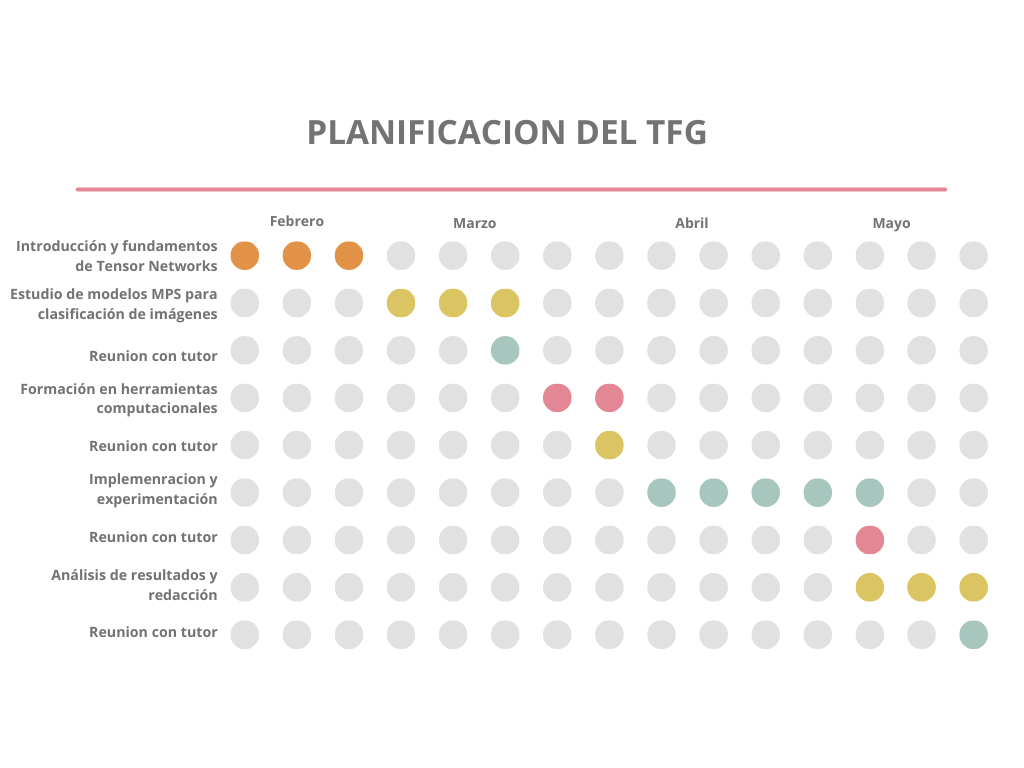
\includegraphics[scale=0.6]{figures/GANTT.png}
    \caption{Planificación por semanas del TFG, cada circulo representa una semana teniendo febrero 3 semanas (porque empiezo el 9 de Febrero), marzo 4 semanas, abril cuatro semanas y por último mayo tendrá otras cuatro semanas. De esta manera se cumplen entre 500 y 600 horas dedicadas al TFG.}
    \label{fig: GANTT}
  \end{minipage}%
}
\end{figure}

\begin{itemize}
\item \textbf{Semanas 1--3: Introducción y fundamentos de Tensor Networks}

Durante las primeras semanas se adquirirán los conocimientos fundamentales y teóricos sobre Tensor Networks. 
\begin{itemize}
\item Estudio de la notación y representaciones básicas de Tensor Networks mediante material audiovisual.
\item Lectura y análisis de artículos científicos relevantes, con especial atención a modelos tensoriales aplicados a clasificación de imágenes.
\item Estudio de apuntes y material teórico relacionado con Tensor Networks y su conexión con la física de sistemas cuánticos.
\end{itemize}

\item \textbf{Semanas 4--6: Estudio de modelos MPS para clasificación de imágenes}

En esta etapa se profundizará en el uso de Matrix Product States como modelos de clasificación de imágenes:
\begin{itemize}
\item Análisis del funcionamiento de clasificadores basados en MPS y estudio de sus fuentes de error.
\item Revisión de implementaciones existentes y comprensión de los procedimientos de entrenamiento y evaluación.
\item Búsqueda y selección de conjuntos de datos adecuados en plataformas como Kaggle o Hugging Face.
\end{itemize}

\item \textbf{Semanas 7--8: Formación en herramientas computacionales}

Durante este periodo se adquirirá el conocimiento práctico necesario para el desarrollo del proyecto:
\begin{itemize}
\item Aprendizaje de comandos básicos de Bash y trabajo en entornos de servidor.
\item Uso de GitHub para el control de versiones y la organización del código.
\item Estudio de buenas prácticas de organización de proyectos y documentación.
\item Aprendizaje en profundidad de PyTorch para la implementación de modelos de inteligencia artificial.
\end{itemize}

\item \textbf{Semanas 9--13: Implementación y experimentación}

En esta fase se llevará a cabo la implementación y entrenamiento de los modelos seleccionados:
\begin{itemize}
\item Implementación de modelos basados en Tensor Networks para clasificación de imágenes.
\item Entrenamiento de los modelos utilizando recursos de computación de altas prestaciones (HPC).
\item Evaluación del rendimiento de los modelos y comparación con modelos de inteligencia artificial convencionales.
\end{itemize}

\item \textbf{Semanas 13--15: Análisis de resultados y redacción}

En la etapa final se realizará el análisis de los resultados obtenidos y la documentación del trabajo:
\begin{itemize}
\item Análisis crítico de los resultados y discusión de las conclusiones.
\item Redacción de la memoria del Trabajo Fin de Grado.
\item Organización final del repositorio de código y preparación de la entrega.
\end{itemize}
\end{itemize}

\section{Recursos requeridos}

A continuación se enumeran los recursos técnicos utilizados para la ejecución del trabajo:

\begin{itemize}
	
	\item Recursos computacionales:
	\begin{itemize}
    		\item Servidor HPC Lorca de la Universidad Europea de Madrid: para el entrenamiento de los modelos con recursos de computación de altas prestaciones.
    		\item Ordenador personal: para el desarrollo, pruebas locales y escritura de la memoria.
	\end{itemize}

	\item Herramientas de software
	\begin{itemize}
   		\item Python (lenguaje de programación principal).
   		 \item PyTorch (framework de deep learning).
    		\item TensorKrowch (librería para implementación de Tensor Networks).
   		 \item NumPy, SciPy, Matplotlib, Seaborn (librerías científicas y de visualización).
    		\item GitHub (control de versiones y gestión del repositorio de código).
    		\item Bash / Linux (gestión del entorno HPC y automatización de trabajos).
    		\item Docker / entornos virtuales (gestión de dependencias y reproducibilidad).
	\end{itemize}

	\item Recursos bibliográficos y de datos:
	\begin{itemize}
   		\item Artículos científicos de referencia (véase sección de Referencias).
   		\item Conjuntos de datos públicos: MNIST, OlivettiFaces (obtenidos de repositorios como Kaggle o Hugging Face).
	\end{itemize}
	
\end{itemize}
